\chapter{Sistema desenvolvido}\label{cap:sistema}
\section{Visão geral e responsabilidades}
O sistema é um protótipo local para preparar coleções fotográficas, receber uma imagem de referência, selecionar uma pessoa quando necessário e retornar fotografias ordenadas. O usuário pode pesquisar por face, por conteúdo global ou, no perfil de pesquisa, pela combinação das duas pistas. Além da consulta, a aplicação permite atualizar índices e remover um álbum cadastrado sem apagar suas fotografias originais.

A implementação é um monólito modular em Python: interface, comandos e avaliação pertencem ao mesmo repositório e não constituem serviços independentes. Uma organização leve por portas e adaptadores separa regras de similaridade, seleção e ranking do acesso a modelos, arquivos e apresentação. \citeonline{Cockburn2005} descreve esse padrão como uma forma de permitir que a mesma aplicação seja acionada por usuários, programas e testes. Aqui, sua adoção é parcial e concreta: funções públicas e formatos de dados representam os contratos, sem uma classe abstrata para cada operação.

O núcleo possui três grupos de responsabilidades. O domínio define similaridade, seleção de face, fusão e métricas. A camada de aplicação compõe os rankings. Adaptadores carregam modelos, leem fotografias e índices, resolvem exclusões e escrevem manifestos. Os pontos de entrada coordenam esses componentes para a interface ou para um protocolo específico. NumPy e pandas ainda aparecem no núcleo; portanto, não se alega independência absoluta de bibliotecas.

\begin{figure}[htbp]\centering
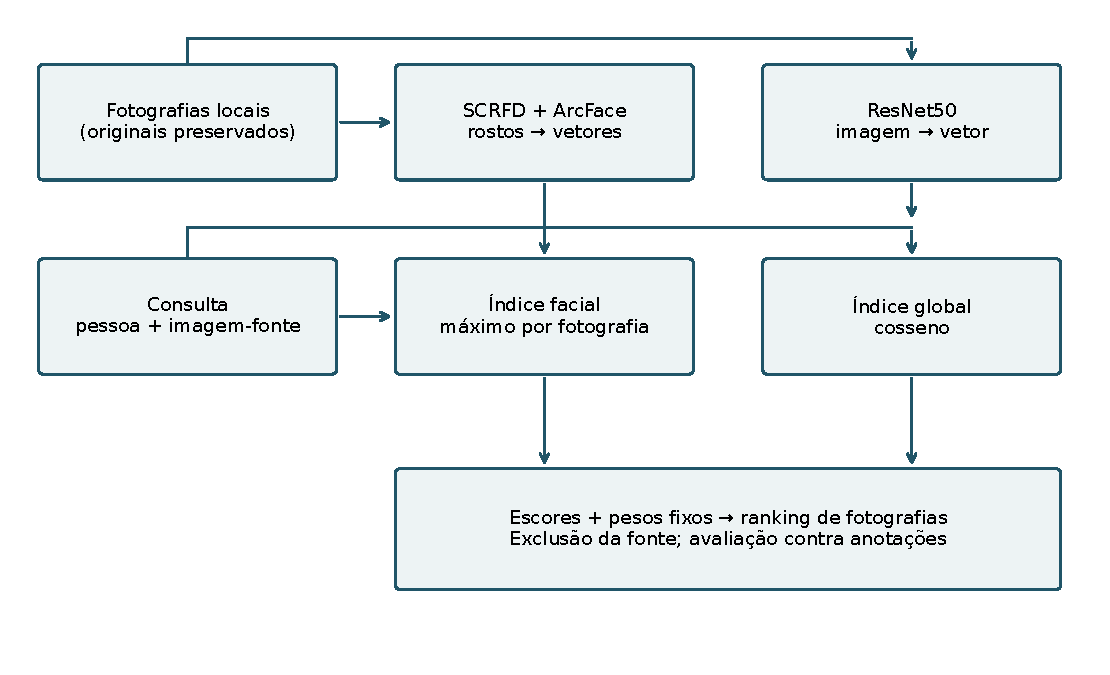
\includegraphics[width=\textwidth]{figuras/fluxo_sistema.pdf}
\caption{Fluxo conceitual da preparação e da recuperação}\label{fig:fluxo}
\fonte{elaboração para esta monografia a partir dos adaptadores e regras documentados; diagrama conceitual, sem fotografias ou saídas simuladas de reconhecimento}
\end{figure}

Na Figura~\ref{fig:fluxo}, as representações facial e global são obtidas a partir das fotografias e utilizadas em operações de busca distintas. O descritor facial caracteriza um rosto; o global caracteriza a imagem após sua transformação de entrada. Os dois são comparados em seus próprios espaços antes da fusão de escores. O diagrama resume responsabilidades, não impõe uma ordem de execução concorrente nem representa serviços de rede.

\section{Preparação dos álbuns e armazenamento}
Preparar uma coleção consiste em percorrer a pasta indicada e suas subpastas, ler os formatos suportados, extrair representações e relacioná-las aos arquivos de origem. A operação não exige mover as fotografias para o repositório. Os índices ficam em uma área própria da aplicação; os originais permanecem no local escolhido pelo usuário. Isso evita duplicação desnecessária, mas significa que preparar um álbum não cria um backup: fotografias movidas ou removidas externamente podem deixar de estar disponíveis.

Cada índice relaciona uma matriz numérica em formato NumPy com metadados em CSV. A linha da matriz deve corresponder à linha indicada nos metadados. No índice global há um vetor por fotografia; no facial podem existir vários vetores associados à mesma imagem. Identificadores e hashes ajudam a verificar consistência e a reconhecer a fotografia consultada, mas não tornam os dados anônimos. Os manifestos registram configuração, versões e impressões digitais dos artefatos.

Os formatos suportados incluem JPEG, PNG, BMP, WebP, HEIC e HEIF. O leitor HEIC/HEIF utiliza a dependência já presente no ambiente de referência. JPEGs excepcionalmente grandes recebem tratamento controlado na leitura global e nas prévias: o limite global de proteção do Pillow permanece ativo, e a exceção admite no máximo 256 megapixels de origem, solicita redução de decodificação de 1/8 por dimensão e limita o resultado a 8 megapixels. Os originais não são regravados. Essa política não altera a leitura facial OpenCV dos JPEGs nem introduz uma exceção geral para outros formatos.

Falhas de leitura e ausência de detecção são registradas como situações distintas. Uma fotografia pode ser lida corretamente e não produzir um rosto detectado. Isso não prova que não existam pessoas nela. No protocolo principal, a imagem ainda participa da galeria global e seu rótulo de relevância continua vindo da anotação, como detalhado no Capítulo~\ref{cap:metodo}.

\section{Extração facial e global}
O adaptador facial utiliza InsightFace 0.2.1 com os pesos do pacote \metodo{buffalo\_l}. Os manifestos identificam \metodo{det\_10g.onnx} para detecção SCRFD e \metodo{w600k\_r50.onnx} para reconhecimento ArcFaceONNX. A dimensão do vetor facial é 512; a detecção é preparada com tamanho de entrada $640\times640$ e limiar padrão 0,5 da biblioteca instalada. A biblioteca alinha a região facial pelos pontos detectados antes de gerar o descritor. Os vetores são normalizados para comparação.

O nome do pacote, isoladamente, não substitui os hashes dos pesos: arquivos e bibliotecas podem mudar ao longo do tempo. A reprodução utilizada registra as versões e os arquivos concretos carregados. O código científico não treina novas identidades, não ajusta pesos e não usa um classificador de atributos como avaliador de identidade. A licença de código e as condições dos modelos são tratadas separadamente \cite{InsightFace}.

No componente global, a ResNet50 de torchvision é carregada com \metodo{DEFAULT}, equivalente a \metodo{IMAGENET1K\_V2} na versão 0.26 \cite{Torchvision}. O extrator remove a camada classificadora final e produz 2.048 componentes após a agregação espacial. O pré-processamento redimensiona com parâmetro 232, aplica recorte central $224\times224$, converte para a escala esperada e normaliza os canais pelas médias $(0{,}485,0{,}456,0{,}406)$ e desvios $(0{,}229,0{,}224,0{,}225)$. O vetor final recebe normalização L2. Portanto, não se extrai uma representação de fundo segmentado ou de cada objeto isolado.

As redes operam em modo de inferência. A indexação global usa lotes e evita o cálculo de gradientes. Reutilizar modelos treinados reduz o escopo de desenvolvimento necessário à comparação, mas traz limitações: não se conhece, nesta pesquisa, a ausência de sobreposição entre todos os dados de avaliação e os acervos usados no pré-treinamento.

\section{Busca e combinação dos escores}
Na busca facial, o descritor da pessoa selecionada é comparado aos rostos indexados. Se uma fotografia contém vários rostos, utiliza-se o maior escore como sua contribuição facial. A regra traduz a intenção de encontrar uma fotografia que contenha ao menos uma ocorrência semelhante à referência, evitando devolver a mesma fotografia repetidamente por diferentes faces.

Na busca global, compara-se o vetor da imagem de consulta com os vetores das imagens da galeria. Na fusão, os escores são remapeados e somados com pesos declarados. Não há concatenação de embeddings, aprendizagem de peso por usuário ou treinamento conjunto de face e cena. A formalização no Capítulo~\ref{cap:metodo} separa a disponibilidade de face de um escore facial válido.

A versão ativa compara os descritores com o acervo carregado em memória; não usa FAISS. Esse desenho permite inspecionar diretamente as regras de ranking no experimento delimitado, mas não demonstra desempenho para acervos arbitrariamente maiores. A quantidade de resultados exibida e a quantidade de imagens indexadas também não são a mesma coisa: retirar um limite de resultados da interface não mede capacidade computacional.

\section{Interface, seleção da pessoa e ciclo do álbum}
O perfil inicial, \emph{Uso pessoal}, oferece a busca nos álbuns preparados e o acesso à gestão de coleções. Quando não existe álbum pronto, orienta a preparação do primeiro. As bases científicas não são escolhidas automaticamente como alternativa. O perfil \emph{Pesquisa} é ativado explicitamente e expõe fusão experimental e índices personalizados.

Ao receber a fotografia de referência, a interface apresenta os rostos detectados com numeração e permite escolher a pessoa. A escolha visual do usuário é necessária em consultas com várias faces: selecionar sempre a maior caixa não representa necessariamente a intenção de busca. Essa operação interativa difere da seleção científica vinculada ao ponto anotado dos olhos em Gallagher.

O fluxo de preparação produz o índice do álbum; atualizar repete a preparação no mesmo destino, substituindo os arquivos gerados e invalidando os caches correspondentes. Se a preparação falhar, o álbum fica marcado como incompleto e não entra na seleção normal de busca. A remoção exige confirmação e é limitada aos índices e registros gerados para o álbum. Caminhos externos, vínculos e conteúdos não reconhecidos bloqueiam a remoção protegida; as fotografias originais não são o alvo dessa rotina.

Os resultados são exibidos em páginas de 24 fotografias. O usuário pode solicitar todos os resultados ou fixar um máximo, sujeito aos filtros do modo escolhido. Alterações apenas de exibição não precisam recalcular o ranking. Mudar a referência, a pessoa, o álbum, os parâmetros ou os índices invalida a busca anterior. Os caches de análise e de índices são limitados; a consulta local recebe nome derivado do conteúdo para evitar colisões entre arquivos de mesmo nome.

O sistema interativo exclui a fotografia de consulta quando reconhecida por caminho ou SHA-256. Já os avaliadores preservam regras próprias de exclusão declaradas em cada protocolo. Em particular, não se deve inferir que o tratamento de duplicatas por hash da interface seja idêntico ao de Holidays. A interface é um meio de uso e exploração, não uma execução automática do experimento.

\section{Execução e limites da demonstração}
No fechamento de 28/09/2026, foi corrigida a seleção de provedores do adaptador facial: no InsightFace 0.2.1, solicitar \metodo{ctx\_id=0} não bastava para ativar CUDA nas sessões ONNX. O adaptador passou a configurar e verificar os provedores de detecção e reconhecimento. Os manifestos atuais registram CUDA e CPU; o segundo pode atender operadores sem implementação na GPU. Isso não equivale a afirmar que todo operador execute em CUDA.

O fechamento registra 93 testes aprovados e aceitação integrada com uma coleção privada. Essa evidência sustenta os caminhos testados, incluindo escolha de pessoa, preparação, atualização, paginação e remoção. Não é uma medida de satisfação, facilidade de aprendizagem, taxa de reconhecimento familiar ou desempenho sob carga. Esta monografia descreve o software consolidado, sem acrescentar uma arquitetura, publicar o sistema na nuvem ou repetir a inferência para a escrita.
